\documentclass[1p]{elsarticle_modified}
%\bibliographystyle{elsarticle-num}

%\usepackage[colorlinks]{hyperref}
%\usepackage{abbrmath_seonhwa} %\Abb, \Ascr, \Acal ,\Abf, \Afrak
\usepackage{amsfonts}
\usepackage{amssymb}
\usepackage{amsmath}
\usepackage{amsthm}
\usepackage{scalefnt}
\usepackage{amsbsy}
\usepackage{kotex}
\usepackage{caption}
\usepackage{subfig}
\usepackage{color}
\usepackage{graphicx}
\usepackage{xcolor} %% white, black, red, green, blue, cyan, magenta, yellow
\usepackage{float}
\usepackage{setspace}
\usepackage{hyperref}

\usepackage{tikz}
\usetikzlibrary{arrows}

\usepackage{multirow}
\usepackage{array} % fixed length table
\usepackage{hhline}

%%%%%%%%%%%%%%%%%%%%%
\makeatletter
\renewcommand*\env@matrix[1][\arraystretch]{%
	\edef\arraystretch{#1}%
	\hskip -\arraycolsep
	\let\@ifnextchar\new@ifnextchar
	\array{*\c@MaxMatrixCols c}}
\makeatother %https://tex.stackexchange.com/questions/14071/how-can-i-increase-the-line-spacing-in-a-matrix
%%%%%%%%%%%%%%%

\usepackage[normalem]{ulem}

\newcommand{\msout}[1]{\ifmmode\text{\sout{\ensuremath{#1}}}\else\sout{#1}\fi}
%SOURCE: \msout is \stkout macro in https://tex.stackexchange.com/questions/20609/strikeout-in-math-mode

\newcommand{\cancel}[1]{
	\ifmmode
	{\color{red}\msout{#1}}
	\else
	{\color{red}\sout{#1}}
	\fi
}

\newcommand{\add}[1]{
	{\color{blue}\uwave{#1}}
}

\newcommand{\replace}[2]{
	\ifmmode
	{\color{red}\msout{#1}}{\color{blue}\uwave{#2}}
	\else
	{\color{red}\sout{#1}}{\color{blue}\uwave{#2}}
	\fi
}

\newcommand{\Sol}{\mathcal{S}} %segment
\newcommand{\D}{D} %diagram
\newcommand{\A}{\mathcal{A}} %arc


%%%%%%%%%%%%%%%%%%%%%%%%%%%%%5 test

\def\sl{\operatorname{\textup{SL}}(2,\Cbb)}
\def\psl{\operatorname{\textup{PSL}}(2,\Cbb)}
\def\quan{\mkern 1mu \triangleright \mkern 1mu}

\theoremstyle{definition}
\newtheorem{thm}{Theorem}[section]
\newtheorem{prop}[thm]{Proposition}
\newtheorem{lem}[thm]{Lemma}
\newtheorem{ques}[thm]{Question}
\newtheorem{cor}[thm]{Corollary}
\newtheorem{defn}[thm]{Definition}
\newtheorem{exam}[thm]{Example}
\newtheorem{rmk}[thm]{Remark}
\newtheorem{alg}[thm]{Algorithm}

\newcommand{\I}{\sqrt{-1}}
\begin{document}

%\begin{frontmatter}
%
%\title{Boundary parabolic representations of knots up to 8 crossings}
%
%%% Group authors per affiliation:
%\author{Yunhi Cho} 
%\address{Department of Mathematics, University of Seoul, Seoul, Korea}
%\ead{yhcho@uos.ac.kr}
%
%
%\author{Seonhwa Kim} %\fnref{s_kim}}
%\address{Center for Geometry and Physics, Institute for Basic Science, Pohang, 37673, Korea}
%\ead{ryeona17@ibs.re.kr}
%
%\author{Hyuk Kim}
%\address{Department of Mathematical Sciences, Seoul National University, Seoul 08826, Korea}
%\ead{hyukkim@snu.ac.kr}
%
%\author{Seokbeom Yoon}
%\address{Department of Mathematical Sciences, Seoul National University, Seoul, 08826,  Korea}
%\ead{sbyoon15@snu.ac.kr}
%
%\begin{abstract}
%We find all boundary parabolic representation of knots up to 8 crossings.
%
%\end{abstract}
%\begin{keyword}
%    \MSC[2010] 57M25 
%\end{keyword}
%
%\end{frontmatter}

%\linenumbers
%\tableofcontents
%
\newcommand\colored[1]{\textcolor{white}{\rule[-0.35ex]{0.8em}{1.4ex}}\kern-0.8em\color{red} #1}%
%\newcommand\colored[1]{\textcolor{white}{ #1}\kern-2.17ex	\textcolor{white}{ #1}\kern-1.81ex	\textcolor{white}{ #1}\kern-2.15ex\color{red}#1	}

{\Large $\underline{12n_{0230}~(K12n_{0230})}$}

\setlength{\tabcolsep}{10pt}
\renewcommand{\arraystretch}{1.6}
\vspace{1cm}\begin{tabular}{m{100pt}>{\centering\arraybackslash}m{274pt}}
\multirow{5}{120pt}{
	\centering
	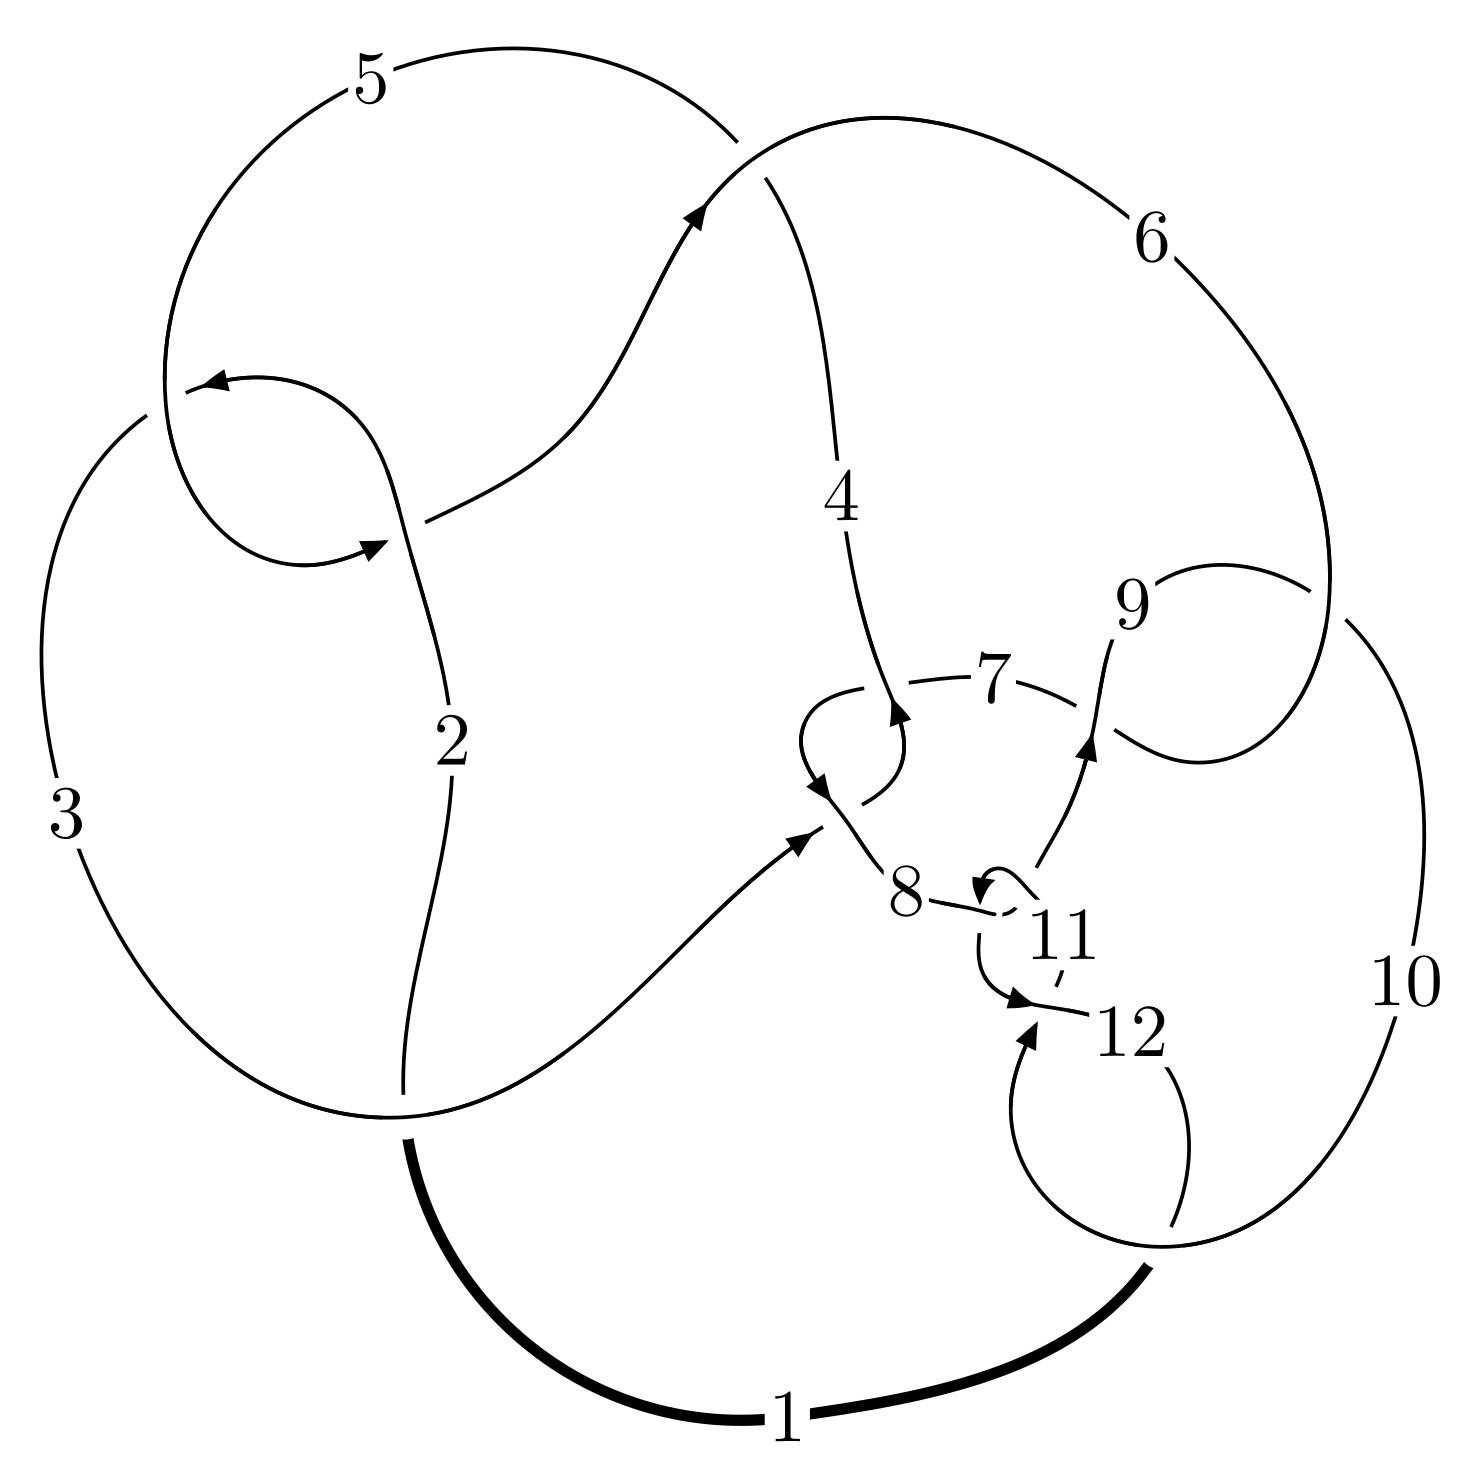
\includegraphics[width=112pt]{../../../GIT/diagram.site/Diagrams/png/2319_12n_0230.png}\\
\ \ \ A knot diagram\footnotemark}&
\allowdisplaybreaks
\textbf{Linearized knot diagam} \\
\cline{2-2}
 &
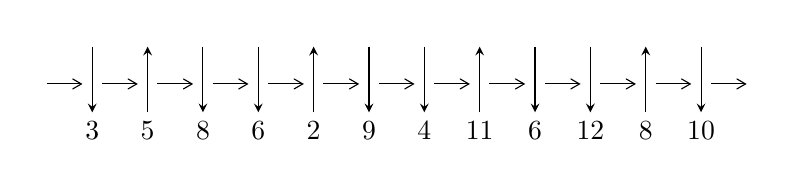
\begin{tikzpicture}[x=20pt, y=17pt]
	% nodes
	\node (C0) at (0, 0) {};
	\node (C1) at (1, 0) {};
	\node (C1U) at (1, +1) {};
	\node (C1D) at (1, -1) {3};

	\node (C2) at (2, 0) {};
	\node (C2U) at (2, +1) {};
	\node (C2D) at (2, -1) {5};

	\node (C3) at (3, 0) {};
	\node (C3U) at (3, +1) {};
	\node (C3D) at (3, -1) {8};

	\node (C4) at (4, 0) {};
	\node (C4U) at (4, +1) {};
	\node (C4D) at (4, -1) {6};

	\node (C5) at (5, 0) {};
	\node (C5U) at (5, +1) {};
	\node (C5D) at (5, -1) {2};

	\node (C6) at (6, 0) {};
	\node (C6U) at (6, +1) {};
	\node (C6D) at (6, -1) {9};

	\node (C7) at (7, 0) {};
	\node (C7U) at (7, +1) {};
	\node (C7D) at (7, -1) {4};

	\node (C8) at (8, 0) {};
	\node (C8U) at (8, +1) {};
	\node (C8D) at (8, -1) {11};

	\node (C9) at (9, 0) {};
	\node (C9U) at (9, +1) {};
	\node (C9D) at (9, -1) {6};

	\node (C10) at (10, 0) {};
	\node (C10U) at (10, +1) {};
	\node (C10D) at (10, -1) {12};

	\node (C11) at (11, 0) {};
	\node (C11U) at (11, +1) {};
	\node (C11D) at (11, -1) {8};

	\node (C12) at (12, 0) {};
	\node (C12U) at (12, +1) {};
	\node (C12D) at (12, -1) {10};
	\node (C13) at (13, 0) {};

	% arrows
	\draw[->,>={angle 60}]
	(C0) edge (C1) (C1) edge (C2) (C2) edge (C3) (C3) edge (C4) (C4) edge (C5) (C5) edge (C6) (C6) edge (C7) (C7) edge (C8) (C8) edge (C9) (C9) edge (C10) (C10) edge (C11) (C11) edge (C12) (C12) edge (C13) ;	\draw[->,>=stealth]
	(C1U) edge (C1D) (C2D) edge (C2U) (C3U) edge (C3D) (C4U) edge (C4D) (C5D) edge (C5U) (C6U) edge (C6D) (C7U) edge (C7D) (C8D) edge (C8U) (C9U) edge (C9D) (C10U) edge (C10D) (C11D) edge (C11U) (C12U) edge (C12D) ;
	\end{tikzpicture} \\
\hhline{~~} \\& 
\textbf{Solving Sequence} \\ \cline{2-2} 
 &
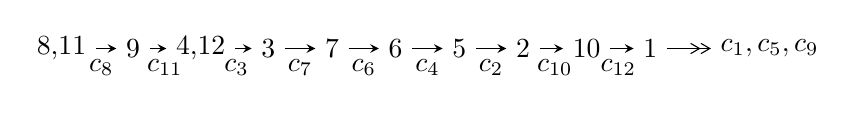
\begin{tikzpicture}[x=23pt, y=7pt]
	% node
	\node (A0) at (-1/8, 0) {8,11};
	\node (A1) at (1, 0) {9};
	\node (A2) at (33/16, 0) {4,12};
	\node (A3) at (25/8, 0) {3};
	\node (A4) at (33/8, 0) {7};
	\node (A5) at (41/8, 0) {6};
	\node (A6) at (49/8, 0) {5};
	\node (A7) at (57/8, 0) {2};
	\node (A8) at (65/8, 0) {10};
	\node (A9) at (73/8, 0) {1};
	\node (C1) at (1/2, -1) {$c_{8}$};
	\node (C2) at (3/2, -1) {$c_{11}$};
	\node (C3) at (21/8, -1) {$c_{3}$};
	\node (C4) at (29/8, -1) {$c_{7}$};
	\node (C5) at (37/8, -1) {$c_{6}$};
	\node (C6) at (45/8, -1) {$c_{4}$};
	\node (C7) at (53/8, -1) {$c_{2}$};
	\node (C8) at (61/8, -1) {$c_{10}$};
	\node (C9) at (69/8, -1) {$c_{12}$};
	\node (A10) at (11, 0) {$c_{1},c_{5},c_{9}$};

	% edge
	\draw[->,>=stealth]	
	(A0) edge (A1) (A1) edge (A2) (A2) edge (A3) (A3) edge (A4) (A4) edge (A5) (A5) edge (A6) (A6) edge (A7) (A7) edge (A8) (A8) edge (A9) ;
	\draw[->>,>={angle 60}]	
	(A9) edge (A10);
\end{tikzpicture} \\ 

\end{tabular} \\

\footnotetext{
The image of knot diagram is generated by the software ``\textbf{Draw programme}" developed by Andrew Bartholomew(\url{http://www.layer8.co.uk/maths/draw/index.htm\#Running-draw}), where we modified some parts for our purpose(\url{https://github.com/CATsTAILs/LinksPainter}).
}\phantom \\ \newline 
\centering \textbf{Ideals for irreducible components\footnotemark of $X_{\text{par}}$} 
 
\begin{align*}
I^u_{1}&=\langle 
- u^7+2 u^6-3 u^5+2 u^4-2 u^3+2 u^2+b- u,\;u^5-2 u^4+2 u^3+a- u,\\
\phantom{I^u_{1}}&\phantom{= \langle  }u^9-3 u^8+6 u^7-7 u^6+7 u^5-7 u^4+6 u^3-4 u^2+u-1\rangle \\
I^u_{2}&=\langle 
130 u^{15}-449 u^{14}+\cdots+1816 b-497,\;-1016 u^{15}+4012 u^{14}+\cdots+1816 a-9397,\\
\phantom{I^u_{2}}&\phantom{= \langle  }u^{16}-4 u^{15}+\cdots+2 u+1\rangle \\
I^u_{3}&=\langle 
b,\;- u^3 a+2 u^2 a- u^3+a^2-2 a u- u^2+3 u-4,\;u^4- u^3+u^2+1\rangle \\
I^u_{4}&=\langle 
- a^3 u-2 a^3-3 a^2- a u+3 b+a+u+5,\;a^4- a^3 u+2 a^3- a^2 u-4 a- u-4,\;u^2+u+1\rangle \\
\\
\end{align*}
\raggedright * 4 irreducible components of $\dim_{\mathbb{C}}=0$, with total 41 representations.\\
\footnotetext{All coefficients of polynomials are rational numbers. But the coefficients are sometimes approximated in decimal forms when there is not enough margin.}
\newpage
\renewcommand{\arraystretch}{1}
\centering \section*{I. $I^u_{1}= \langle - u^7+2 u^6-3 u^5+2 u^4-2 u^3+2 u^2+b- u,\;u^5-2 u^4+2 u^3+a- u,\;u^9-3 u^8+\cdots+u-1 \rangle$}
\flushleft \textbf{(i) Arc colorings}\\
\begin{tabular}{m{7pt} m{180pt} m{7pt} m{180pt} }
\flushright $a_{8}=$&$\begin{pmatrix}1\\0\end{pmatrix}$ \\
\flushright $a_{11}=$&$\begin{pmatrix}0\\u\end{pmatrix}$ \\
\flushright $a_{9}=$&$\begin{pmatrix}1\\- u^2\end{pmatrix}$ \\
\flushright $a_{4}=$&$\begin{pmatrix}- u^5+2 u^4-2 u^3+u\\u^7-2 u^6+3 u^5-2 u^4+2 u^3-2 u^2+u\end{pmatrix}$ \\
\flushright $a_{12}=$&$\begin{pmatrix}u\\u\end{pmatrix}$ \\
\flushright $a_{3}=$&$\begin{pmatrix}u^7-2 u^6+2 u^5-2 u^2+2 u\\u^7-2 u^6+3 u^5-2 u^4+2 u^3-2 u^2+u\end{pmatrix}$ \\
\flushright $a_{7}=$&$\begin{pmatrix}- u^5+2 u^4-2 u^3+2 u^2- u+2\\- u^5- u^3- u\end{pmatrix}$ \\
\flushright $a_{6}=$&$\begin{pmatrix}- u^7+2 u^6-4 u^5+4 u^4-4 u^3+4 u^2-2 u+2\\u^8-3 u^7+5 u^6-6 u^5+5 u^4-6 u^3+4 u^2-2 u+1\end{pmatrix}$ \\
\flushright $a_{5}=$&$\begin{pmatrix}- u^8+2 u^7-3 u^6+2 u^5- u^4+2 u^3-2 u^2+2 u-1\\- u^8+2 u^7-4 u^6+4 u^5-4 u^4+4 u^3-2 u^2+2 u\end{pmatrix}$ \\
\flushright $a_{2}=$&$\begin{pmatrix}- u^8+4 u^7-7 u^6+8 u^5-5 u^4+4 u^3-4 u^2+2 u-1\\- u^8+3 u^7-5 u^6+6 u^5-5 u^4+6 u^3-4 u^2+2 u-1\end{pmatrix}$ \\
\flushright $a_{10}=$&$\begin{pmatrix}u^3\\u^3+u\end{pmatrix}$ \\
\flushright $a_{1}=$&$\begin{pmatrix}u^5+u\\u^5+u^3+u\end{pmatrix}$\\&\end{tabular}
\flushleft \textbf{(ii) Obstruction class $= -1$}\\~\\
\flushleft \textbf{(iii) Cusp Shapes $= 8 u^8-24 u^7+48 u^6-56 u^5+48 u^4-32 u^3+8 u^2-6$}\\~\\
\newpage\renewcommand{\arraystretch}{1}
\flushleft \textbf{(iv) u-Polynomials at the component}\newline \\
\begin{tabular}{m{50pt}|m{274pt}}
Crossings & \hspace{64pt}u-Polynomials at each crossing \\
\hline $$\begin{aligned}c_{1},c_{4},c_{10}\\c_{12}\end{aligned}$$&$\begin{aligned}
&u^9+3 u^8+8 u^7+5 u^6+u^5-15 u^4-20 u^3-18 u^2-7 u-1
\end{aligned}$\\
\hline $$\begin{aligned}c_{2},c_{5},c_{8}\\c_{11}\end{aligned}$$&$\begin{aligned}
&u^9+3 u^8+6 u^7+7 u^6+7 u^5+7 u^4+6 u^3+4 u^2+u+1
\end{aligned}$\\
\hline $$\begin{aligned}c_{3},c_{6},c_{7}\\c_{9}\end{aligned}$$&$\begin{aligned}
&u^9- u^8-2 u^7+9 u^6+3 u^5+17 u^4+6 u^3+4 u^2- u+1
\end{aligned}$\\
\hline
\end{tabular}\\~\\
\newpage\renewcommand{\arraystretch}{1}
\flushleft \textbf{(v) Riley Polynomials at the component}\newline \\
\begin{tabular}{m{50pt}|m{274pt}}
Crossings & \hspace{64pt}Riley Polynomials at each crossing \\
\hline $$\begin{aligned}c_{1},c_{4},c_{10}\\c_{12}\end{aligned}$$&$\begin{aligned}
&y^9+7 y^8+36 y^7+41 y^6-75 y^5-191 y^4-144 y^3-74 y^2+13 y-1
\end{aligned}$\\
\hline $$\begin{aligned}c_{2},c_{5},c_{8}\\c_{11}\end{aligned}$$&$\begin{aligned}
&y^9+3 y^8+8 y^7+5 y^6+y^5-15 y^4-20 y^3-18 y^2-7 y-1
\end{aligned}$\\
\hline $$\begin{aligned}c_{3},c_{6},c_{7}\\c_{9}\end{aligned}$$&$\begin{aligned}
&y^9-5 y^8+28 y^7-47 y^6-315 y^5-319 y^4-124 y^3-62 y^2-7 y-1
\end{aligned}$\\
\hline
\end{tabular}\\~\\
\newpage\flushleft \textbf{(vi) Complex Volumes and Cusp Shapes}
$$\begin{array}{c|c|c}  
\text{Solutions to }I^u_{1}& \I (\text{vol} + \sqrt{-1}CS) & \text{Cusp shape}\\
 \hline 
\begin{aligned}
u &= -0.461481 + 0.837544 I \\
a &= -2.45813 + 3.10206 I \\
b &= -0.213712 - 0.318134 I\end{aligned}
 & -0.13903 - 3.77297 I & \phantom{-}10.5564 + 43.0949 I \\ \hline\begin{aligned}
u &= -0.461481 - 0.837544 I \\
a &= -2.45813 - 3.10206 I \\
b &= -0.213712 + 0.318134 I\end{aligned}
 & -0.13903 + 3.77297 I & \phantom{-}10.5564 - 43.0949 I \\ \hline\begin{aligned}
u &= \phantom{-}0.736616 + 0.869782 I \\
a &= \phantom{-}0.787377 + 0.049850 I \\
b &= \phantom{-}0.073895 - 1.113510 I\end{aligned}
 & \phantom{-}7.66695 + 5.59873 I & \phantom{-}4.90357 - 6.20498 I \\ \hline\begin{aligned}
u &= \phantom{-}0.736616 - 0.869782 I \\
a &= \phantom{-}0.787377 - 0.049850 I \\
b &= \phantom{-}0.073895 + 1.113510 I\end{aligned}
 & \phantom{-}7.66695 - 5.59873 I & \phantom{-}4.90357 + 6.20498 I \\ \hline\begin{aligned}
u &= \phantom{-}1.15634\phantom{ +0.000000I} \\
a &= -0.427626\phantom{ +0.000000I} \\
b &= \phantom{-}2.18402\phantom{ +0.000000I}\end{aligned}
 & -4.53774\phantom{ +0.000000I} & -0.758800\phantom{ +0.000000I} \\ \hline\begin{aligned}
u &= -0.102202 + 0.554352 I \\
a &= -0.092950 + 0.960014 I \\
b &= \phantom{-}0.439047 + 0.496789 I\end{aligned}
 & -0.75640 - 1.26978 I & -6.33576 + 4.10506 I \\ \hline\begin{aligned}
u &= -0.102202 - 0.554352 I \\
a &= -0.092950 - 0.960014 I \\
b &= \phantom{-}0.439047 - 0.496789 I\end{aligned}
 & -0.75640 + 1.26978 I & -6.33576 - 4.10506 I \\ \hline\begin{aligned}
u &= \phantom{-}0.74890 + 1.31534 I \\
a &= -1.52248 - 1.01662 I \\
b &= -1.89124 + 1.45525 I\end{aligned}
 & -11.9049 + 13.3161 I & -3.74481 - 5.95110 I \\ \hline\begin{aligned}
u &= \phantom{-}0.74890 - 1.31534 I \\
a &= -1.52248 + 1.01662 I \\
b &= -1.89124 - 1.45525 I\end{aligned}
 & -11.9049 - 13.3161 I & -3.74481 + 5.95110 I\\
 \hline 
 \end{array}$$\newpage\newpage\renewcommand{\arraystretch}{1}
\centering \section*{II. $I^u_{2}= \langle 130 u^{15}-449 u^{14}+\cdots+1816 b-497,\;-1016 u^{15}+4012 u^{14}+\cdots+1816 a-9397,\;u^{16}-4 u^{15}+\cdots+2 u+1 \rangle$}
\flushleft \textbf{(i) Arc colorings}\\
\begin{tabular}{m{7pt} m{180pt} m{7pt} m{180pt} }
\flushright $a_{8}=$&$\begin{pmatrix}1\\0\end{pmatrix}$ \\
\flushright $a_{11}=$&$\begin{pmatrix}0\\u\end{pmatrix}$ \\
\flushright $a_{9}=$&$\begin{pmatrix}1\\- u^2\end{pmatrix}$ \\
\flushright $a_{4}=$&$\begin{pmatrix}0.559471 u^{15}-2.20925 u^{14}+\cdots+18.6828 u+5.17456\\-0.0715859 u^{15}+0.247247 u^{14}+\cdots-3.57654 u+0.273678\end{pmatrix}$ \\
\flushright $a_{12}=$&$\begin{pmatrix}u\\u\end{pmatrix}$ \\
\flushright $a_{3}=$&$\begin{pmatrix}0.487885 u^{15}-1.96200 u^{14}+\cdots+15.1063 u+5.44824\\-0.0715859 u^{15}+0.247247 u^{14}+\cdots-3.57654 u+0.273678\end{pmatrix}$ \\
\flushright $a_{7}=$&$\begin{pmatrix}0.198789 u^{15}-0.833700 u^{14}+\cdots+12.0231 u-1.85518\\0.106278 u^{15}-0.327643 u^{14}+\cdots+2.14152 u+0.192731\end{pmatrix}$ \\
\flushright $a_{6}=$&$\begin{pmatrix}0.226322 u^{15}-0.976872 u^{14}+\cdots+14.0430 u-1.62390\\0.0666300 u^{15}-0.271476 u^{14}+\cdots+2.10297 u+0.159692\end{pmatrix}$ \\
\flushright $a_{5}=$&$\begin{pmatrix}0.318282 u^{15}-1.18007 u^{14}+\cdots+4.34416 u+4.72357\\-0.0440529 u^{15}+0.229075 u^{14}+\cdots-3.93172 u+0.00495595\end{pmatrix}$ \\
\flushright $a_{2}=$&$\begin{pmatrix}-0.101872 u^{15}+0.529736 u^{14}+\cdots-12.1233 u+4.14427\\-0.0666300 u^{15}+0.271476 u^{14}+\cdots-2.10297 u-0.159692\end{pmatrix}$ \\
\flushright $a_{10}=$&$\begin{pmatrix}u^3\\u^3+u\end{pmatrix}$ \\
\flushright $a_{1}=$&$\begin{pmatrix}u^5+u\\u^5+u^3+u\end{pmatrix}$\\&\end{tabular}
\flushleft \textbf{(ii) Obstruction class $= -1$}\\~\\
\flushleft \textbf{(iii) Cusp Shapes $= -\frac{1189}{1816} u^{15}+\frac{4957}{1816} u^{14}+\cdots-\frac{61683}{1816} u-\frac{2179}{908}$}\\~\\
\newpage\renewcommand{\arraystretch}{1}
\flushleft \textbf{(iv) u-Polynomials at the component}\newline \\
\begin{tabular}{m{50pt}|m{274pt}}
Crossings & \hspace{64pt}u-Polynomials at each crossing \\
\hline $$\begin{aligned}c_{1},c_{4},c_{10}\\c_{12}\end{aligned}$$&$\begin{aligned}
&u^{16}+14 u^{15}+\cdots+88 u+1
\end{aligned}$\\
\hline $$\begin{aligned}c_{2},c_{5},c_{8}\\c_{11}\end{aligned}$$&$\begin{aligned}
&u^{16}+4 u^{15}+\cdots-2 u+1
\end{aligned}$\\
\hline $$\begin{aligned}c_{3},c_{6},c_{7}\\c_{9}\end{aligned}$$&$\begin{aligned}
&u^{16}-2 u^{15}+\cdots-128 u+256
\end{aligned}$\\
\hline
\end{tabular}\\~\\
\newpage\renewcommand{\arraystretch}{1}
\flushleft \textbf{(v) Riley Polynomials at the component}\newline \\
\begin{tabular}{m{50pt}|m{274pt}}
Crossings & \hspace{64pt}Riley Polynomials at each crossing \\
\hline $$\begin{aligned}c_{1},c_{4},c_{10}\\c_{12}\end{aligned}$$&$\begin{aligned}
&y^{16}-18 y^{15}+\cdots-2472 y+1
\end{aligned}$\\
\hline $$\begin{aligned}c_{2},c_{5},c_{8}\\c_{11}\end{aligned}$$&$\begin{aligned}
&y^{16}+14 y^{15}+\cdots+88 y+1
\end{aligned}$\\
\hline $$\begin{aligned}c_{3},c_{6},c_{7}\\c_{9}\end{aligned}$$&$\begin{aligned}
&y^{16}-30 y^{15}+\cdots+540672 y+65536
\end{aligned}$\\
\hline
\end{tabular}\\~\\
\newpage\flushleft \textbf{(vi) Complex Volumes and Cusp Shapes}
$$\begin{array}{c|c|c}  
\text{Solutions to }I^u_{2}& \I (\text{vol} + \sqrt{-1}CS) & \text{Cusp shape}\\
 \hline 
\begin{aligned}
u &= -0.363037 + 0.817564 I \\
a &= -0.689592 + 0.163353 I \\
b &= -0.232606 + 0.296439 I\end{aligned}
 & -0.31180 - 1.54577 I & -2.35937 + 4.98634 I \\ \hline\begin{aligned}
u &= -0.363037 - 0.817564 I \\
a &= -0.689592 - 0.163353 I \\
b &= -0.232606 - 0.296439 I\end{aligned}
 & -0.31180 + 1.54577 I & -2.35937 - 4.98634 I \\ \hline\begin{aligned}
u &= -0.479632 + 1.036130 I \\
a &= \phantom{-}1.70605 - 1.00375 I \\
b &= \phantom{-}0.266035 + 0.849001 I\end{aligned}
 & -0.679161\phantom{ +0.000000I} &                  -6
-0.644221 + 0. 10   I\phantom{ +0.000000I} \\ \hline\begin{aligned}
u &= -0.479632 - 1.036130 I \\
a &= \phantom{-}1.70605 + 1.00375 I \\
b &= \phantom{-}0.266035 - 0.849001 I\end{aligned}
 & -0.679161\phantom{ +0.000000I} &                  -6
-0.644221 + 0. 10   I\phantom{ +0.000000I} \\ \hline\begin{aligned}
u &= \phantom{-}0.735167 + 1.044790 I \\
a &= -0.615383 + 0.536646 I \\
b &= \phantom{-}0.72302 + 1.24109 I\end{aligned}
 & \phantom{-}7.14404\phantom{ +0.000000I} &                  -6
-0.483738 + 0. 10   I\phantom{ +0.000000I} \\ \hline\begin{aligned}
u &= \phantom{-}0.735167 - 1.044790 I \\
a &= -0.615383 - 0.536646 I \\
b &= \phantom{-}0.72302 - 1.24109 I\end{aligned}
 & \phantom{-}7.14404\phantom{ +0.000000I} &                  -6
-0.483738 + 0. 10   I\phantom{ +0.000000I} \\ \hline\begin{aligned}
u &= \phantom{-}1.264520 + 0.320297 I \\
a &= \phantom{-}0.438859 + 0.167437 I \\
b &= -2.28152 - 0.82827 I\end{aligned}
 & -8.81126 - 6.26912 I & -2.84932 + 2.54582 I \\ \hline\begin{aligned}
u &= \phantom{-}1.264520 - 0.320297 I \\
a &= \phantom{-}0.438859 - 0.167437 I \\
b &= -2.28152 + 0.82827 I\end{aligned}
 & -8.81126 + 6.26912 I & -2.84932 - 2.54582 I \\ \hline\begin{aligned}
u &= \phantom{-}0.61669 + 1.39802 I \\
a &= \phantom{-}1.61861 + 0.89803 I \\
b &= \phantom{-}2.33600 - 1.15509 I\end{aligned}
 & -8.81126 + 6.26912 I & -2.84932 - 2.54582 I \\ \hline\begin{aligned}
u &= \phantom{-}0.61669 - 1.39802 I \\
a &= \phantom{-}1.61861 - 0.89803 I \\
b &= \phantom{-}2.33600 + 1.15509 I\end{aligned}
 & -8.81126 - 6.26912 I & -2.84932 + 2.54582 I\\
 \hline 
 \end{array}$$\newpage$$\begin{array}{c|c|c}  
\text{Solutions to }I^u_{2}& \I (\text{vol} + \sqrt{-1}CS) & \text{Cusp shape}\\
 \hline 
\begin{aligned}
u &= -0.14859 + 1.53192 I \\
a &= \phantom{-}0.687769 - 1.077410 I \\
b &= \phantom{-}1.29707 - 2.19154 I\end{aligned}
 & -5.68794\phantom{ +0.000000I} & -5.90825 + 0. I\phantom{ +0.000000I} \\ \hline\begin{aligned}
u &= -0.14859 - 1.53192 I \\
a &= \phantom{-}0.687769 + 1.077410 I \\
b &= \phantom{-}1.29707 + 2.19154 I\end{aligned}
 & -5.68794\phantom{ +0.000000I} & -5.90825 + 0. I\phantom{ +0.000000I} \\ \hline\begin{aligned}
u &= \phantom{-}0.41065 + 1.67828 I \\
a &= -1.61714 - 0.65436 I \\
b &= -3.40684 + 0.49631 I\end{aligned}
 & -15.4295\phantom{ +0.000000I} & -5.54640 + 0. I\phantom{ +0.000000I} \\ \hline\begin{aligned}
u &= \phantom{-}0.41065 - 1.67828 I \\
a &= -1.61714 + 0.65436 I \\
b &= -3.40684 - 0.49631 I\end{aligned}
 & -15.4295\phantom{ +0.000000I} & -5.54640 + 0. I\phantom{ +0.000000I} \\ \hline\begin{aligned}
u &= -0.035772 + 0.140099 I \\
a &= \phantom{-}4.97083 + 2.67001 I \\
b &= \phantom{-}0.298852 - 0.519319 I\end{aligned}
 & -0.31180 + 1.54577 I & -2.35937 - 4.98634 I \\ \hline\begin{aligned}
u &= -0.035772 - 0.140099 I \\
a &= \phantom{-}4.97083 - 2.67001 I \\
b &= \phantom{-}0.298852 + 0.519319 I\end{aligned}
 & -0.31180 - 1.54577 I & -2.35937 + 4.98634 I\\
 \hline 
 \end{array}$$\newpage\newpage\renewcommand{\arraystretch}{1}
\centering \section*{III. $I^u_{3}= \langle b,\;- u^3 a+2 u^2 a- u^3+a^2-2 a u- u^2+3 u-4,\;u^4- u^3+u^2+1 \rangle$}
\flushleft \textbf{(i) Arc colorings}\\
\begin{tabular}{m{7pt} m{180pt} m{7pt} m{180pt} }
\flushright $a_{8}=$&$\begin{pmatrix}1\\0\end{pmatrix}$ \\
\flushright $a_{11}=$&$\begin{pmatrix}0\\u\end{pmatrix}$ \\
\flushright $a_{9}=$&$\begin{pmatrix}1\\- u^2\end{pmatrix}$ \\
\flushright $a_{4}=$&$\begin{pmatrix}a\\0\end{pmatrix}$ \\
\flushright $a_{12}=$&$\begin{pmatrix}u\\u\end{pmatrix}$ \\
\flushright $a_{3}=$&$\begin{pmatrix}a\\0\end{pmatrix}$ \\
\flushright $a_{7}=$&$\begin{pmatrix}1\\0\end{pmatrix}$ \\
\flushright $a_{6}=$&$\begin{pmatrix}u^2+1\\- u^3+u^2+1\end{pmatrix}$ \\
\flushright $a_{5}=$&$\begin{pmatrix}2 u^2 a+a u+2 a\\-2 u^3 a+2 u^2 a+a u+2 a\end{pmatrix}$ \\
\flushright $a_{2}=$&$\begin{pmatrix}- u^3+u^2+a-2 u-1\\u^3- u^2-1\end{pmatrix}$ \\
\flushright $a_{10}=$&$\begin{pmatrix}u^3\\u^3+u\end{pmatrix}$ \\
\flushright $a_{1}=$&$\begin{pmatrix}- u^2-1\\u^3- u^2-1\end{pmatrix}$\\&\end{tabular}
\flushleft \textbf{(ii) Obstruction class $= 1$}\\~\\
\flushleft \textbf{(iii) Cusp Shapes $= u^3 a-3 u^2 a+u^3- a u-3 u^2- a+u-2$}\\~\\
\newpage\renewcommand{\arraystretch}{1}
\flushleft \textbf{(iv) u-Polynomials at the component}\newline \\
\begin{tabular}{m{50pt}|m{274pt}}
Crossings & \hspace{64pt}u-Polynomials at each crossing \\
\hline $$\begin{aligned}c_{1},c_{4},c_{5}\end{aligned}$$&$\begin{aligned}
&(u^2- u+1)^4
\end{aligned}$\\
\hline $$\begin{aligned}c_{2}\end{aligned}$$&$\begin{aligned}
&(u^2+u+1)^4
\end{aligned}$\\
\hline $$\begin{aligned}c_{3},c_{7}\end{aligned}$$&$\begin{aligned}
&u^8
\end{aligned}$\\
\hline $$\begin{aligned}c_{6},c_{10}\end{aligned}$$&$\begin{aligned}
&(u^4- u^3+3 u^2-2 u+1)^2
\end{aligned}$\\
\hline $$\begin{aligned}c_{8}\end{aligned}$$&$\begin{aligned}
&(u^4- u^3+u^2+1)^2
\end{aligned}$\\
\hline $$\begin{aligned}c_{9},c_{12}\end{aligned}$$&$\begin{aligned}
&(u^4+u^3+3 u^2+2 u+1)^2
\end{aligned}$\\
\hline $$\begin{aligned}c_{11}\end{aligned}$$&$\begin{aligned}
&(u^4+u^3+u^2+1)^2
\end{aligned}$\\
\hline
\end{tabular}\\~\\
\newpage\renewcommand{\arraystretch}{1}
\flushleft \textbf{(v) Riley Polynomials at the component}\newline \\
\begin{tabular}{m{50pt}|m{274pt}}
Crossings & \hspace{64pt}Riley Polynomials at each crossing \\
\hline $$\begin{aligned}c_{1},c_{2},c_{4}\\c_{5}\end{aligned}$$&$\begin{aligned}
&(y^2+y+1)^4
\end{aligned}$\\
\hline $$\begin{aligned}c_{3},c_{7}\end{aligned}$$&$\begin{aligned}
&y^8
\end{aligned}$\\
\hline $$\begin{aligned}c_{6},c_{9},c_{10}\\c_{12}\end{aligned}$$&$\begin{aligned}
&(y^4+5 y^3+7 y^2+2 y+1)^2
\end{aligned}$\\
\hline $$\begin{aligned}c_{8},c_{11}\end{aligned}$$&$\begin{aligned}
&(y^4+y^3+3 y^2+2 y+1)^2
\end{aligned}$\\
\hline
\end{tabular}\\~\\
\newpage\flushleft \textbf{(vi) Complex Volumes and Cusp Shapes}
$$\begin{array}{c|c|c}  
\text{Solutions to }I^u_{3}& \I (\text{vol} + \sqrt{-1}CS) & \text{Cusp shape}\\
 \hline 
\begin{aligned}
u &= -0.351808 + 0.720342 I \\
a &= -1.73811 + 1.68562 I \\
b &= \phantom{-0.000000 } 0\end{aligned}
 & -0.211005 + 0.614778 I & \phantom{-}1.30302 + 4.44028 I \\ \hline\begin{aligned}
u &= -0.351808 + 0.720342 I \\
a &= \phantom{-}2.32885 + 0.66243 I \\
b &= \phantom{-0.000000 } 0\end{aligned}
 & -0.21101 - 3.44499 I & -3.64182 + 2.68374 I \\ \hline\begin{aligned}
u &= -0.351808 - 0.720342 I \\
a &= -1.73811 - 1.68562 I \\
b &= \phantom{-0.000000 } 0\end{aligned}
 & -0.211005 - 0.614778 I & \phantom{-}1.30302 - 4.44028 I \\ \hline\begin{aligned}
u &= -0.351808 - 0.720342 I \\
a &= \phantom{-}2.32885 - 0.66243 I \\
b &= \phantom{-0.000000 } 0\end{aligned}
 & -0.21101 + 3.44499 I & -3.64182 - 2.68374 I \\ \hline\begin{aligned}
u &= \phantom{-}0.851808 + 0.911292 I \\
a &= \phantom{-}0.156525 - 0.382204 I \\
b &= \phantom{-0.000000 } 0\end{aligned}
 & \phantom{-}6.79074 + 1.13408 I & -1.68800 - 4.61015 I \\ \hline\begin{aligned}
u &= \phantom{-}0.851808 + 0.911292 I \\
a &= \phantom{-}0.252736 + 0.326656 I \\
b &= \phantom{-0.000000 } 0\end{aligned}
 & \phantom{-}6.79074 + 5.19385 I & -4.47320 - 2.03656 I \\ \hline\begin{aligned}
u &= \phantom{-}0.851808 - 0.911292 I \\
a &= \phantom{-}0.156525 + 0.382204 I \\
b &= \phantom{-0.000000 } 0\end{aligned}
 & \phantom{-}6.79074 - 1.13408 I & -1.68800 + 4.61015 I \\ \hline\begin{aligned}
u &= \phantom{-}0.851808 - 0.911292 I \\
a &= \phantom{-}0.252736 - 0.326656 I \\
b &= \phantom{-0.000000 } 0\end{aligned}
 & \phantom{-}6.79074 - 5.19385 I & -4.47320 + 2.03656 I\\
 \hline 
 \end{array}$$\newpage\newpage\renewcommand{\arraystretch}{1}
\centering \section*{IV. $I^u_{4}= \langle - a^3 u-2 a^3-3 a^2- a u+3 b+a+u+5,\;a^4- a^3 u+2 a^3- a^2 u-4 a- u-4,\;u^2+u+1 \rangle$}
\flushleft \textbf{(i) Arc colorings}\\
\begin{tabular}{m{7pt} m{180pt} m{7pt} m{180pt} }
\flushright $a_{8}=$&$\begin{pmatrix}1\\0\end{pmatrix}$ \\
\flushright $a_{11}=$&$\begin{pmatrix}0\\u\end{pmatrix}$ \\
\flushright $a_{9}=$&$\begin{pmatrix}1\\u+1\end{pmatrix}$ \\
\flushright $a_{4}=$&$\begin{pmatrix}a\\\frac{1}{3} a^3 u+\frac{1}{3} a u+\cdots-\frac{1}{3} a-\frac{5}{3}\end{pmatrix}$ \\
\flushright $a_{12}=$&$\begin{pmatrix}u\\u\end{pmatrix}$ \\
\flushright $a_{3}=$&$\begin{pmatrix}\frac{1}{3} a^3 u+\frac{1}{3} a u+\cdots+\frac{2}{3} a-\frac{5}{3}\\\frac{1}{3} a^3 u+\frac{1}{3} a u+\cdots-\frac{1}{3} a-\frac{5}{3}\end{pmatrix}$ \\
\flushright $a_{7}=$&$\begin{pmatrix}\frac{1}{3} a^3 u-\frac{2}{3} a^2 u+\cdots- a-\frac{4}{3}\\\frac{2}{3} a^3 u+\frac{2}{3} a^2 u+\cdots+\frac{4}{3} a^2+\frac{1}{3}\end{pmatrix}$ \\
\flushright $a_{6}=$&$\begin{pmatrix}\frac{1}{3} a^3 u-\frac{2}{3} a^2 u+\cdots- a-\frac{4}{3}\\\frac{2}{3} a^3 u+\frac{2}{3} a^2 u+\cdots+\frac{4}{3} a^2+\frac{1}{3}\end{pmatrix}$ \\
\flushright $a_{5}=$&$\begin{pmatrix}\frac{2}{3} a^3 u+\frac{4}{3} a^2 u+\cdots-\frac{1}{3} a+1\\-\frac{1}{3} a^3 u-\frac{1}{3} a^2 u+\cdots-\frac{2}{3} a^2+\frac{4}{3}\end{pmatrix}$ \\
\flushright $a_{2}=$&$\begin{pmatrix}a^3 u+a^3+2 a^2-2 a u- a-3 u-3\\\frac{2}{3} a^3 u+\frac{2}{3} a^2 u+\cdots+\frac{4}{3} a^2+\frac{1}{3}\end{pmatrix}$ \\
\flushright $a_{10}=$&$\begin{pmatrix}1\\u+1\end{pmatrix}$ \\
\flushright $a_{1}=$&$\begin{pmatrix}-1\\0\end{pmatrix}$\\&\end{tabular}
\flushleft \textbf{(ii) Obstruction class $= 1$}\\~\\
\flushleft \textbf{(iii) Cusp Shapes $= -\frac{5}{3} a^3 u-\frac{7}{3} a^3- a^2 u-5 a^2+\frac{4}{3} a u+\frac{8}{3} a+\frac{5}{3} u+\frac{13}{3}$}\\~\\
\newpage\renewcommand{\arraystretch}{1}
\flushleft \textbf{(iv) u-Polynomials at the component}\newline \\
\begin{tabular}{m{50pt}|m{274pt}}
Crossings & \hspace{64pt}u-Polynomials at each crossing \\
\hline $$\begin{aligned}c_{1},c_{3},c_{4}\end{aligned}$$&$\begin{aligned}
&(u^4- u^3+3 u^2-2 u+1)^2
\end{aligned}$\\
\hline $$\begin{aligned}c_{2}\end{aligned}$$&$\begin{aligned}
&(u^4- u^3+u^2+1)^2
\end{aligned}$\\
\hline $$\begin{aligned}c_{5}\end{aligned}$$&$\begin{aligned}
&(u^4+u^3+u^2+1)^2
\end{aligned}$\\
\hline $$\begin{aligned}c_{6},c_{9}\end{aligned}$$&$\begin{aligned}
&u^8
\end{aligned}$\\
\hline $$\begin{aligned}c_{7}\end{aligned}$$&$\begin{aligned}
&(u^4+u^3+3 u^2+2 u+1)^2
\end{aligned}$\\
\hline $$\begin{aligned}c_{8},c_{12}\end{aligned}$$&$\begin{aligned}
&(u^2+u+1)^4
\end{aligned}$\\
\hline $$\begin{aligned}c_{10},c_{11}\end{aligned}$$&$\begin{aligned}
&(u^2- u+1)^4
\end{aligned}$\\
\hline
\end{tabular}\\~\\
\newpage\renewcommand{\arraystretch}{1}
\flushleft \textbf{(v) Riley Polynomials at the component}\newline \\
\begin{tabular}{m{50pt}|m{274pt}}
Crossings & \hspace{64pt}Riley Polynomials at each crossing \\
\hline $$\begin{aligned}c_{1},c_{3},c_{4}\\c_{7}\end{aligned}$$&$\begin{aligned}
&(y^4+5 y^3+7 y^2+2 y+1)^2
\end{aligned}$\\
\hline $$\begin{aligned}c_{2},c_{5}\end{aligned}$$&$\begin{aligned}
&(y^4+y^3+3 y^2+2 y+1)^2
\end{aligned}$\\
\hline $$\begin{aligned}c_{6},c_{9}\end{aligned}$$&$\begin{aligned}
&y^8
\end{aligned}$\\
\hline $$\begin{aligned}c_{8},c_{10},c_{11}\\c_{12}\end{aligned}$$&$\begin{aligned}
&(y^2+y+1)^4
\end{aligned}$\\
\hline
\end{tabular}\\~\\
\newpage\flushleft \textbf{(vi) Complex Volumes and Cusp Shapes}
$$\begin{array}{c|c|c}  
\text{Solutions to }I^u_{4}& \I (\text{vol} + \sqrt{-1}CS) & \text{Cusp shape}\\
 \hline 
\begin{aligned}
u &= -0.500000 + 0.866025 I \\
a &= -0.715307 - 0.631577 I \\
b &= -0.395123 + 0.506844 I\end{aligned}
 & -0.211005 - 0.614778 I & \phantom{-}1.30302 - 4.44028 I \\ \hline\begin{aligned}
u &= -0.500000 + 0.866025 I \\
a &= \phantom{-}1.248740 + 0.225872 I \\
b &= -0.10488 + 1.55249 I\end{aligned}
 & \phantom{-}6.79074 + 1.13408 I & -1.68800 - 4.61015 I \\ \hline\begin{aligned}
u &= -0.500000 + 0.866025 I \\
a &= -1.44025 - 0.04422 I \\
b &= -0.10488 - 1.55249 I\end{aligned}
 & \phantom{-}6.79074 - 5.19385 I & -4.47320 + 2.03656 I \\ \hline\begin{aligned}
u &= -0.500000 + 0.866025 I \\
a &= -1.59319 + 1.31595 I \\
b &= -0.395123 - 0.506844 I\end{aligned}
 & -0.21101 - 3.44499 I & -3.64182 + 2.68374 I \\ \hline\begin{aligned}
u &= -0.500000 - 0.866025 I \\
a &= -0.715307 + 0.631577 I \\
b &= -0.395123 - 0.506844 I\end{aligned}
 & -0.211005 + 0.614778 I & \phantom{-}1.30302 + 4.44028 I \\ \hline\begin{aligned}
u &= -0.500000 - 0.866025 I \\
a &= \phantom{-}1.248740 - 0.225872 I \\
b &= -0.10488 - 1.55249 I\end{aligned}
 & \phantom{-}6.79074 - 1.13408 I & -1.68800 + 4.61015 I \\ \hline\begin{aligned}
u &= -0.500000 - 0.866025 I \\
a &= -1.44025 + 0.04422 I \\
b &= -0.10488 + 1.55249 I\end{aligned}
 & \phantom{-}6.79074 + 5.19385 I & -4.47320 - 2.03656 I \\ \hline\begin{aligned}
u &= -0.500000 - 0.866025 I \\
a &= -1.59319 - 1.31595 I \\
b &= -0.395123 + 0.506844 I\end{aligned}
 & -0.21101 + 3.44499 I & -3.64182 - 2.68374 I\\
 \hline 
 \end{array}$$\newpage
\newpage\renewcommand{\arraystretch}{1}
\centering \section*{ V. u-Polynomials}
\begin{tabular}{m{50pt}|m{274pt}}
Crossings & \hspace{64pt}u-Polynomials at each crossing \\
\hline $$\begin{aligned}c_{1},c_{4},c_{10}\end{aligned}$$&$\begin{aligned}
&(u^2- u+1)^4(u^4- u^3+3 u^2-2 u+1)^2\\
&\cdot(u^9+3 u^8+8 u^7+5 u^6+u^5-15 u^4-20 u^3-18 u^2-7 u-1)\\
&\cdot(u^{16}+14 u^{15}+\cdots+88 u+1)
\end{aligned}$\\
\hline $$\begin{aligned}c_{2},c_{8}\end{aligned}$$&$\begin{aligned}
&(u^2+u+1)^4(u^4- u^3+u^2+1)^2\\
&\cdot(u^9+3 u^8+6 u^7+7 u^6+7 u^5+7 u^4+6 u^3+4 u^2+u+1)\\
&\cdot(u^{16}+4 u^{15}+\cdots-2 u+1)
\end{aligned}$\\
\hline $$\begin{aligned}c_{3},c_{6}\end{aligned}$$&$\begin{aligned}
&u^8(u^4- u^3+3 u^2-2 u+1)^2\\
&\cdot(u^9- u^8-2 u^7+9 u^6+3 u^5+17 u^4+6 u^3+4 u^2- u+1)\\
&\cdot(u^{16}-2 u^{15}+\cdots-128 u+256)
\end{aligned}$\\
\hline $$\begin{aligned}c_{5},c_{11}\end{aligned}$$&$\begin{aligned}
&(u^2- u+1)^4(u^4+u^3+u^2+1)^2\\
&\cdot(u^9+3 u^8+6 u^7+7 u^6+7 u^5+7 u^4+6 u^3+4 u^2+u+1)\\
&\cdot(u^{16}+4 u^{15}+\cdots-2 u+1)
\end{aligned}$\\
\hline $$\begin{aligned}c_{7},c_{9}\end{aligned}$$&$\begin{aligned}
&u^8(u^4+u^3+3 u^2+2 u+1)^2\\
&\cdot(u^9- u^8-2 u^7+9 u^6+3 u^5+17 u^4+6 u^3+4 u^2- u+1)\\
&\cdot(u^{16}-2 u^{15}+\cdots-128 u+256)
\end{aligned}$\\
\hline $$\begin{aligned}c_{12}\end{aligned}$$&$\begin{aligned}
&(u^2+u+1)^4(u^4+u^3+3 u^2+2 u+1)^2\\
&\cdot(u^9+3 u^8+8 u^7+5 u^6+u^5-15 u^4-20 u^3-18 u^2-7 u-1)\\
&\cdot(u^{16}+14 u^{15}+\cdots+88 u+1)
\end{aligned}$\\
\hline
\end{tabular}\newpage\renewcommand{\arraystretch}{1}
\centering \section*{ VI. Riley Polynomials}
\begin{tabular}{m{50pt}|m{274pt}}
Crossings & \hspace{64pt}Riley Polynomials at each crossing \\
\hline $$\begin{aligned}c_{1},c_{4},c_{10}\\c_{12}\end{aligned}$$&$\begin{aligned}
&(y^2+y+1)^4(y^4+5 y^3+7 y^2+2 y+1)^2\\
&\cdot(y^9+7 y^8+36 y^7+41 y^6-75 y^5-191 y^4-144 y^3-74 y^2+13 y-1)\\
&\cdot(y^{16}-18 y^{15}+\cdots-2472 y+1)
\end{aligned}$\\
\hline $$\begin{aligned}c_{2},c_{5},c_{8}\\c_{11}\end{aligned}$$&$\begin{aligned}
&(y^2+y+1)^4(y^4+y^3+3 y^2+2 y+1)^2\\
&\cdot(y^9+3 y^8+8 y^7+5 y^6+y^5-15 y^4-20 y^3-18 y^2-7 y-1)\\
&\cdot(y^{16}+14 y^{15}+\cdots+88 y+1)
\end{aligned}$\\
\hline $$\begin{aligned}c_{3},c_{6},c_{7}\\c_{9}\end{aligned}$$&$\begin{aligned}
&y^8(y^4+5 y^3+7 y^2+2 y+1)^2\\
&\cdot(y^9-5 y^8+28 y^7-47 y^6-315 y^5-319 y^4-124 y^3-62 y^2-7 y-1)\\
&\cdot(y^{16}-30 y^{15}+\cdots+540672 y+65536)
\end{aligned}$\\
\hline
\end{tabular}
\vskip 2pc
\end{document}